\documentclass[a4paper, 12pt]{article}


\usepackage[portuges]{babel}
\usepackage[utf8]{inputenc}

\usepackage{indentfirst}
\usepackage{graphicx}
\usepackage{float}% ante frescura de imagens
\usepackage{multicol,lipsum}
\usepackage{mathptmx}
\usepackage{ragged2e}% testo justificado
\usepackage{setspace} % espaçamento entre linhas
\usepackage{amsmath} % números complexos
\usepackage{amssymb} % mesure angle
\usepackage{siunitx} %simbolo micro

\usepackage{geometry}
\geometry{ a4paper, total={170mm,257mm}, left=30mm, right = 25mm, top=30mm, bottom = 20mm }

% padrao 1.5 de espacamento entre linhas
\setstretch{1.5}
\begin{document}

%\maketitle

\begin{titlepage}
	\begin{center}
		\Huge{Universidade Federal de Uberlândia}\\
	   \textbf{\LARGE{}}\\
		%\title{{\large{Título}}}
		\vspace{3,5cm}
	\end{center}

	\begin{flushleft}
		\begin{tabbing}
			Aluno: Henrique Santos de Lima - 11811ETE016\\
			Professor: Wellington Maycon Santos Bernardes\\
	\end{tabbing}
 \end{flushleft}
	\vspace{1cm}

	\begin{center}
		\vspace{\fill}
			 Novembro\\
		 2019
			\end{center}
\end{titlepage}
%%%%%%%%%%%%%%%%%%%%%%%%%%%%%%%%%%%%%%%%%%%%%%%%%%%%%%%%%%%

% % % % % % % % %FOLHA DE ROSTO % % % % % % % % % %

\begin{titlepage}
	\begin{center}

	%\begin{figure}[!ht]
	%\centering
	%\includegraphics[width=2cm]{c:/ufba.jpg}
	%\end{figure}

		\Huge{Universidade Federal de Uberlândia}\\
	\vspace{15pt}

        \vspace{85pt}

		\textbf{\LARGE{Relatório de Experimental de Circuitos Elétricos 2}}
		\title{\large{Título}}
	%	\large{Modelo\\
     %   		Validação do modelo clássico}

	\end{center}
\vspace{1,5cm}

\begin{flushright}
\begin{list}{}{
    \setlength{\leftmargin}{4.5cm}
    \setlength{\rightmargin}{0cm}
    \setlength{\labelwidth}{0pt}
    \setlength{\labelsep}{\leftmargin}}

    \item
    Circuitos Trifásicos desequilibrados
    \begin{list}{}{
    \setlength{\leftmargin}{0cm}
    \setlength{\rightmargin}{0cm}
    \setlength{\labelwidth}{0pt}
    \setlength{\labelsep}{\leftmargin}}
    \item Aluno:  Henrique Santos de Lima - 11811ETE016\
    \item Professor : Wellington Maycon Santos Bernardes\
\end{list}
   \end{list}
\end{flushright}
\vspace{1cm}
\begin{center}
		\vspace{\fill}
			 Novembro\\
		 2019
			\end{center}
\end{titlepage}

\tableofcontents

\thispagestyle{empty}

\newpage
%\pagenumbering{times new romam}
% % % % % % % % % % % % % % % % % % % % % % % % % % %
\section{Objetivos}

\justifying
    Medir as potência ativa e reativa usando o método dos dois wattímetros, averiguar se este método funciona comparando com os valores obtidos analiticamente.
\section{Introdução}

\justifying
  O Wattímetro analógico mostra com sua ponteira o resultado da parte real da multiplicação
  da tensão lida com o conjugado da corrente lida. \(W = \Re\{V \ast I^\ast\}\) . Para uma mesma fase essa leitura possui significado físico de potencia ativa, porém dependendo da ligação a medida apresentada pode não ter um significado físico.

  O método dos dois wattímetros consiste em usar dois wattímetros para realizar a medida da potencia trifásica. Para realizar essa medida deve-se :
    \begin{itemize}
        \item Escolher duas fases.
        \item Medir a corrente que passa na  fase escolhida e a tensão entre a mesma e a fase não \\ escolhida.
        \item Fazer o mesmo com a segunda Fase escolhida.
    \end{itemize}
    Exemplo:\\
    \begin{figure}[H]
            \centering % para centralizarmos a figura
            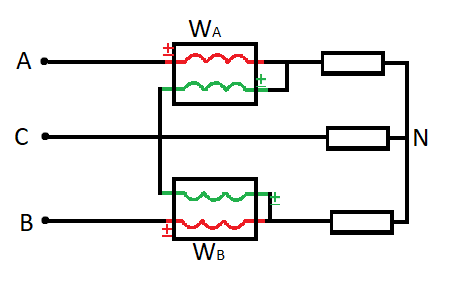
\includegraphics[]{montagem_2watt_A+C.png}
            \caption{montagem usando 2 wattímetros}
    \end{figure}

    Para entender qual significado físico de cada medição:
        Considerando a sequencia ABC temos:
\[ \begin{split}
&\begin{bmatrix} V_{AB}\\ V_{BC}\\ V_{CA} \end{bmatrix} = V_L \angle \theta \begin{bmatrix} 1\\  \alpha^2\\  \alpha \end{bmatrix}\\
&\begin{bmatrix} V_{AN}\\ V_{BN}\\ V_{CN} \end{bmatrix} = \frac{V_L}{\sqrt{3}} \measuredangle{( \theta-30^\circ)} \begin{bmatrix} 1\\  \alpha^2\\  \alpha \end{bmatrix} \\
&\begin{bmatrix} I_{A}\\ I_{B}\\ I_{C} \end{bmatrix} = I_L\measuredangle{(( \theta-30^\circ) - \theta_z)} \begin{bmatrix} 1\\  \alpha^2\\  \alpha \end{bmatrix}
\end{split}
\]

\[\begin{split}
W_1 &= \Re\{V_{AC} \ast I_A^\ast\}\\
W_1 &= \Re\{-\alpha \ast V_L\measuredangle{\theta} \ast I_L\measuredangle{(-\theta+30^\circ+\theta_z)}\}\\
W_1 &= \Re\{V_L\ast I_L\measuredangle{(\theta-\theta+30^\circ+\theta_z - 60^\circ)}\}\\
W_1 &= \Re\{V_L\ast I_L\measuredangle{(\theta_z - 30^\circ)}\}\\
W_1 &= V_L\ast I_L \ast \cos(\theta _z - 30^\circ)
\end{split}\]
\[
\begin{split}
    W_2 &= \Re\{V_{BC} \ast I_B^\ast\}\\
    W_2 &= \Re\{(\alpha^2 \ast V_L\measuredangle{\theta})\ast (\alpha^2 \ast I_L\measuredangle{(\theta-30^\circ-\theta_z)}\})^\ast\\
    W_2 &= \Re\{(V_L\measuredangle{\{\theta-120^\circ}\})\ast (\ast I_L\measuredangle{(-\theta+30^\circ+\theta_z+120^\circ)}\})\\
    W_2 &= \Re\{V_L\ast I_L\measuredangle{(\theta-\theta+30^\circ+\theta_z-120^\circ + 120^\circ)}\}\\
    W_2 &= \Re\{V_L\ast I_L\measuredangle{(\theta_z + 30^\circ)}\}\\
    W_2 &= V_L\ast I_L \ast \cos(\theta _z + 30^\circ)
\end{split}\]

De modo que $W_1 + W_2 = \sqrt{3}*V_L*I_L*\cos(\theta_z) =P_{3\phi} $ que é a potencia trifásica da carga, e $W_1 - W_2 = V_L*I_L*\sin(\theta_z) = \frac{Q_{3\phi}}{\sqrt{3}}$

Para determinar qual wattímetro corresponde ao $W_1$ e $W_2$ utiliza-se o método abaixo:
\newpage
\begin{itemize}
            \item Desenhar a sequencia de fase
        \end{itemize}
        \begin{figure}[H]
             \centering % para centralizarmos a figura
            \includegraphics[width=0.5\columnwidth]{definindo_w1_e_w2_p1.png}
            \caption{Desenho para sequencia ABC}
        \end{figure}
        \begin{itemize}
            \item Destacar fase que não possui Wattímetro
        \end{itemize}
        \begin{figure}[H]
             \centering % para centralizarmos a figura
            \includegraphics[width=0.5\columnwidth]{definindo_w1_e_w2_p2.png}
            \caption{Fase C destacada}
        \end{figure}

        \newpage
        \begin{itemize}
            \item Girar no sentido Horário, o primeiro encontrado é o $W_1$ e o segundo é o $W_2$
        \end{itemize}
        \begin{figure}[H]
             \centering % para centralizarmos a figura
            \includegraphics[width=0.5\columnwidth]{definindo_w1_e_w2_p3.png}
            \caption{$W_A$ foi encontrado primeiro, logo $W_A = W_1$ e $W_B = W_2$}
        \end{figure}
\newpage
\section{Preparação}
    \subsection{Materiais e ferramentas}
        \begin{itemize}
            \item Regulador de tensão(Varivolt)
            \item Resistores banana de 50\(\Omega\)
            \item Indutor de 160 mH
            \item Capacitor de 45.9 \si{\micro}F
            \item Medidor Trifásico Kron Mult-K
            \item Amperímetro analógico AC
            \item Wattímetro analógico
        \end{itemize}
    \subsection{Montagem}
    \subsubsection{Ligação em Estrela}
       \begin{figure}[H]
            \centering % para centralizarmos a figura
            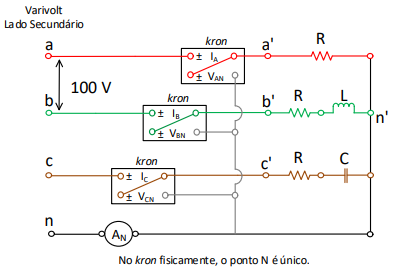
\includegraphics[width = 15cm]{montagem1.png}
            \caption{circuito em estrela a ser montado}
        \end{figure}
        Para realizar a montagem deve seguir a figura 5, antes de iniciar a montagem certifique-se que o circuito esteja desligado.
          \begin{figure}[H]
            \centering % para centralizarmos a figura
           \includegraphics[width= 14cm]{my_montagem1.jpeg}
            \caption{circuito estrela montado}
         \end{figure}

    \subsubsection{Ligação em Delta}
        \begin{figure}[H]
            \centering % para centralizarmos a figura
            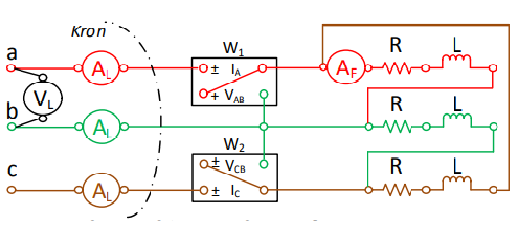
\includegraphics[width= 15cm]{montagem2.png}
            \caption{circuito em delta a ser montado}
            \label{figura:montada}
        \end{figure}

         Para realizar a montagem deve seguir a figura 7, antes de iniciar a montagem certifique-se que o circuito esteja desligado.
        \begin{figure}[H]
            \centering % para centralizarmos a figura
            \includegraphics[width= 14cm]{my_montagem2.jpeg}
            \caption{circuito delta montado}
        \end{figure}



\newpage
\section{Análise sobre segurança}
    \mbox{}
    \justifying
    Antes de montar o experimento é importante o uso de equipamentos de proteção, estar com calça, sapatos fechados, sem acessórios metálicos e se o cabelo for grande, este deve estar preso.

    A bancada deve estar desenergizada durante a montagem. Durante o experimento não ter contato com nenhum fio ou elemento energizado do circuito além do risco de choque elétrico. Certifique-se de que os equipamentos estão na escala adequada para realizar as medições.

    Para movimentar os indutores pegue pela parte inferior evitando riscos de que se desprenda e caia, assim evitando lesões e dano ao dispositivo. Deixe os capacitores na horizontal para que
    fique melhor apoiado na bancada, este é muito leve e pode cair com facilidade.

    Realizar as medidas em um tempo curto evitando que o circuito fique energizado por um longo período de tempo, pois os resistores estarão dissipando potência assim esquentando.

   Deve-se manter uma distância segura do circuito quando o mesmo está energizado assim evitando queimaduras e choque elétrico.


\newpage
\section{Análise}
    \justifying
    \subsection{Dados}
        \subsubsection{Ligação em estrela}
        \justifying

    \begin{table}[H]
         \centering
        \begin{tabular}{|c|c|c|c|c|c|c|}
              \hline %linha horizontal
                  Sequencia & V$_L$[V] & I$_L$[A] & fp & P$_{3\phi}$[W] & Q$_{3\phi}$[Var] & S$_{3\phi}$[VA] \\
              \hline %linha horizontal
           ABC & 100 & 0.6 & 0.62 & 67.46 & 84.18 & 107.70     \\
              \hline %linha horizontal
           CBA & 100 & 0.6 & 0.62 & 67.02 & 83.59 & 107.35     \\
              \hline %linha horizontal
        \end{tabular}
        \caption{Medidas Para circuito em Estrela obtida pelo equipamento Kron}
    \end{table}
    \begin{table}[H]
         \centering
        \begin{tabular}{|c|c|c|c|}
              \hline %linha horizontal
                  Sequencia & w$_1$[W] & w$_2$[W] & $W_1 + W_2$ \\
              \hline %linha horizontal
           ABC & 5 & 55 & 60     \\
              \hline %linha horizontal
           CBA & 55 & 5 & 60     \\
              \hline %linha horizontal
        \end{tabular}
        \caption{Medidas Para circuito em Estrela}
    \end{table}

    Para Sequencia ABC $W_2$ corresponde ao $W_1$ teórico então, temos que:

    \[\begin{split}
        Q_{3\phi} & = \sqrt{3}\ast(w_2 - w_1) \\
        Q_{3\phi} & = \sqrt{3}\ast(55 - 5 ) \\
        Q_{3\phi} & = 86.6
        \end{split}
    \]

    Para Sequencia CBA $W_1$ corresponde ao $W_1$ teórico então, temos que:
       \[\begin{split}
        Q_{3\phi} & = \sqrt{3}\ast(w_1 - w_2) \\
        Q_{3\phi} & = \sqrt{3}\ast(55 - 5 ) \\
        Q_{3\phi} & = 86.6
        \end{split}
    \]

        \subsubsection{Ligação em delta}
        \justifying
    \begin{table}[H]
         \centering
        \begin{tabular}{|c|c|c|c|c|c|c|c|}
              \hline %linha horizontal
                  Sequencia & V$_L$[V] & I$_L$[A] & I$_f$[A] & fp & P$_{3\phi}$[W] & Q$_{3\phi}$[Var] & S$_{3\phi}$[VA] \\
              \hline %linha horizontal
           ABC & 81 & 1.8 & 1 & 0.658 & 168.44 & 193.01 & 257.95     \\
              \hline %linha horizontal
           CBA & 80 & 1.8 & 1 & 0.657 & 164 & 188.29 & 249.89     \\
              \hline %linha horizontal
        \end{tabular}
        \caption{Medidas Para circuito em Delta obtidas pelo equipamento Kron}
    \end{table}

    \begin{table}[H]
         \centering
        \begin{tabular}{|c|c|c|c|}
              \hline %linha horizontal
                  Sequencia & w$_1$[W] & w$_2$[W] & $W_1 + W_2$ \\
              \hline %linha horizontal
           ABC & 115 & 35 & 150     \\
              \hline %linha horizontal
           CBA & 15 & 140 & 155     \\
              \hline %linha horizontal
        \end{tabular}
        \caption{Medidas Para circuito em Delta}
    \end{table}
 Para Sequencia ABC $W_2$ corresponde ao $W_1$ teórico então, temos que:

    \[\begin{split}
        Q_{3\phi} & = \sqrt{3}\ast(w_2 - w_1) \\
        Q_{3\phi} & = \sqrt{3}\ast(35 - 115 ) \\
        Q_{3\phi} & = -138.6 \text{ V}_{ar}
        \end{split}
    \]

    Para Sequencia CBA $W_1$ corresponde ao $W_1$ teórico então, temos que:
       \[\begin{split}
        Q_{3\phi} & = \sqrt{3}\ast(w_1 - w_2) \\
        Q_{3\phi} & = \sqrt{3}\ast(15 - 140 ) \\
        Q_{3\phi} & = -216.5 \text{ V}_{ar}
        \end{split}
    \]

    \subsection{Questões}
        \justifying
    - Para os sistemas das Figuras 1 e 2, ao ser ligado, o que aconteceu com os wattímetros
$W_1$ e $W_2$ quando a sequência de fases foi invertida? Algum deles marcou valor
negativo? Explique. Encontre as potências usando as leituras.\\
R: Ao mudar a sequencia os wattímetros trocaram as leituras. Nenhum marcou e leitura negativa. O Angulo $\theta _z$ de ambas as cargas é menor que $60^\circ$ e a ligação estava correta  por isso não houve medição negativa. Potencia calculada acima.

- Encontre o valor das leituras dos wattímetros usando as expressões analíticas.\\
Para circuito estrela:\\

  \[\begin{split}
        &W_1 = V_L\ast I_L \ast \cos(\theta _z + 30^\circ) \\
        &W_2 = V_L\ast I_L \ast \cos(\theta _z - 30^\circ)\\
        &\cos(\theta) = 0.62 \implies \theta = 51.68 ^\circ\\
        &W_1 = 8.68\\
        &W_2 = 55.76
    \end{split}
    \]
Para circuito delta:\\

  \[\begin{split}
        &W_1 = V_L\ast I_L \ast \cos(\theta _z + 30^\circ) \\
        &W_2 = V_L\ast I_L \ast \cos(\theta _z - 30^\circ)\\
        &\cos(\theta) = 0.658 \implies \theta = -48.85 ^\circ\\
        &W_1 = 136.28\\
        &W_2 = 27.85
    \end{split}
    \]

- Mostre através de um diagrama fasorial que de acordo com as polaridades das bobinas
de corrente e de potencial a leitura do wattímetro analógico é positiva para um ângulo $\left| \theta_z \right|$ menor que 60º.Mostre que a leitura será negativa se  for maior que 60º.\\
R: Se $\left|\theta_z\right| < 60^\circ$ então $\left |\theta_z + 30^\circ\right| < 90^\circ$ e
$\left| \theta_z - 30^\circ \right| < 90^\circ$ assim para $\theta < 90$, $\cos(\theta) > 0$ , ambas leituras serão positivas.\\
Se $\left|\theta_z\right| > 60^\circ$ então $\left |\theta_z + 30^\circ\right| > 90^\circ$ e
$\left| \theta_z - 30^\circ \right| < 90^\circ$ assim para $\theta > 90$, $\cos(\theta) < 0$, uma das leituras será negativa.






- Mostre através de um diagrama fasorial que se a polaridade de uma das bobinas não
for seguida a leitura terá um sinal oposto ao correto.\\
R: Pela definição caso uma  das medidas fique errada, será lido a medida com angulo somado 180. conforme as figuras abaixo mostram. As figuras foram feita a partir de um código[1] em javaScript escrito pelo autor deste relatório.
\begin{figure}[H]
            \centering % para centralizarmos a figura
           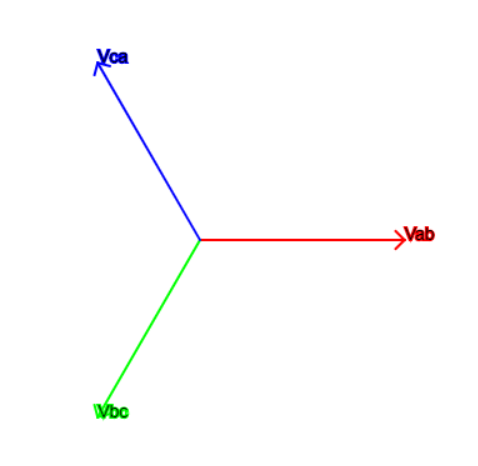
\includegraphics[width=0.7\columnwidth]{fasores.png}
            \caption{Fasores com a medição correta}
    \end{figure}
\begin{figure}[H]
            \centering % para centralizarmos a figura
           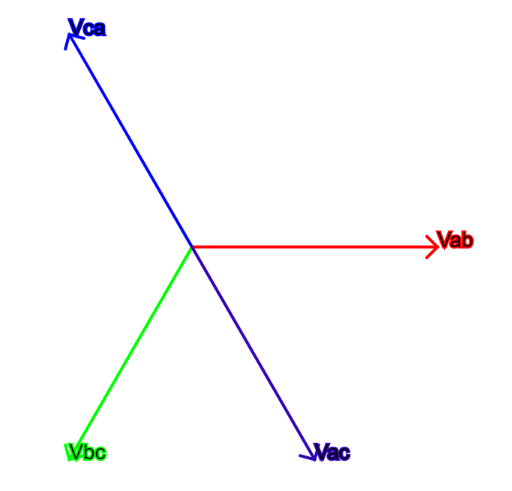
\includegraphics[width=0.7\columnwidth]{fasores2.png}
            \caption{Caso troque a medição $V_{ca}$ por $V_{ac}$ gerando uma leitura negativa}
    \end{figure}

       O mesmo acontece caso a bobina de corrente for invertida.
       \begin{figure}[H]
            \centering % para centralizarmos a figura
           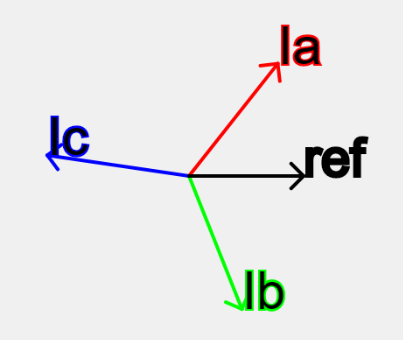
\includegraphics[width=0.7\columnwidth]{fasoresI1.png}
            \caption{Fasores de corrente com a medição correta}
    \end{figure}
\begin{figure}[H]
            \centering % para centralizarmos a figura
           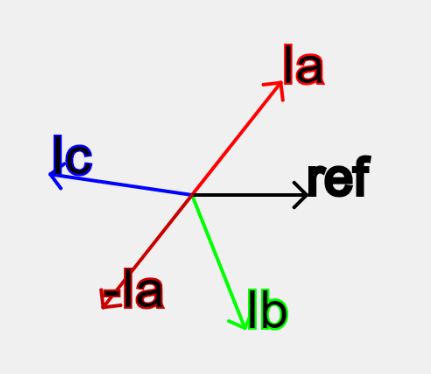
\includegraphics[width=0.7\columnwidth]{fasoresI2.png}
            \caption{Caso troque a medição $I_{a}$ por $-I_a$ gerando uma leitura negativa}
    \end{figure}

\newpage
\section{Simulação}
    \justifying
    \begin{figure}[H]
            \centering % para centralizarmos a figura
           \includegraphics[width=0.7\columnwidth]{simulacao/estrelaabc.png}
            \caption{Simulação em estrela ABC}
    \end{figure}
     \begin{figure}[H]
            \centering % para centralizarmos a figura
           \includegraphics[width=0.7\columnwidth]{simulacao/estrelacba.png}
            \caption{Simulação em estrela CBA}
    \end{figure}
     \begin{figure}[H]
            \centering % para centralizarmos a figura
           \includegraphics[width=0.7\columnwidth]{simulacao/simulacaodelta.png}
            \caption{Simulação em delta ABC}
    \end{figure}
     \begin{figure}[H]
            \centering % para centralizarmos a figura
           \includegraphics[width=0.7\columnwidth]{simulacao/simulacaodeltacba.png}
            \caption{Simulação em estrela CBA}
    \end{figure}
     \begin{table}[H]
         \centering
        \begin{tabular}{|c|c|c|c|c|c|}
              \hline %linha horizontal
                  Sequência & V$_L$[V] & I$_L$[A] & w$_1$[W] & w$_2$[W] & $W_1 + W_2$ \\
              \hline %linha horizontal
           ABC & 80 & 1.8 & 28.1 & 140 & 168     \\
              \hline %linha horizontal
           CBA & 80 & 1.8 & 140 & 28.1 & 168     \\
              \hline %linha horizontal
        \end{tabular}
        \caption{Medidas Simuladas  Para circuito em Delta}
    \end{table}

    \begin{table}[H]
         \centering
        \begin{tabular}{|c|c|c|c|c|c|}
              \hline %linha horizontal
                  Sequência & V$_L$[V] & I$_L$[A] & w$_1$[W] & w$_2$[W] & $W_1 + W_2$ \\
              \hline %linha horizontal
           ABC & 100 & 0.7 & 12.3 & 69.1 & 81.4     \\
              \hline %linha horizontal
           CBA & 100 & 0.7 & 69.1 & 12.3 & 81.4     \\
              \hline %linha horizontal
        \end{tabular}
        \caption{Medidas Simuladas Para circuito em Estrela}
    \end{table}






\newpage
\section{Conclusão}
\justifying
   A medição de potencia trifásica usando o método dos dois wattímetros é importante para conhecimentos didáticos porém não é comumente utilizado em meios práticos. Com o desenvolvimento da tecnologia foram feitos equipamentos digitais mais precisos e mais fáceis de manusear, estes também realizam outras medições.
   \begin{figure}[H]
            \centering % para centralizarmos a figura
           \includegraphics[width=0.7\columnwidth]{pttr.jpg}
            \caption{Analisador de potência trifásica digital [2]}
    \end{figure}

    Os valores analíticos foram levemente diferentes dos obtidos experimentalmente, quando é feito os cálculos despreza-se os efeitos das bobinas.

    Foi observado que ao trocar as sequencias de fases as medições inverteram, porém para quando o circuito era capacitivo as medições inverteram e  foram diferentes, que leva a levantar a hipótese que os capacitores possuíam uma diferença considerável  fazendo o circuito distanciar de um circuito perfeitamente equilibrado.

    A simulação mostrou que ao invertei a sequencia de fase as medições dos wattímetros mudam, este também comprovando a teoria.

    O método mostrou funcionar independente da ligação (estrela ou delta) e independente do tipo da carga (capacitiva ou indutiva) bastando ser equilibrada.

\newpage
\section*{Referencias}
\justifying
\noindent
ALEXANDER, C.K.; SADIKU, M.N. Fundamentos de Circuitos Elétricos. 5ª ed.
Porto Alegre: Mc Graw-Hill, 2015\\

\noindent
[1] - LIMA, H.S.; Desenhando Fasores https://xx220xx.github.io/FASORES/index.html acesso em 28/10/2018 \\

\noindent
[2] Analisador de potência trifásico PCE-PA 8000 - https://www.pce-medidores.com.pt/fichas-dados/analisador-potencia-trifasico-pce-pa-8000.htm acesso em 28/10/2018
\end{document}



